\subsection{Forretningsmodel}

Halvorsen ApS er et lokalt tømmerfirma i Vissenbjerg, der lige nu har 9 ansatte: 6 svende, 2 lærlinge og en sekretær.

Firmaet laver arbejde for private, andre virksomheder og det offentlige.
Lige nu arbejder de hovedsageligt for Entrepenør Per Petersen.

Firmaet bruger en basal virksomhedsform fra Mintzbergs model, da tømmermesteren har direkte kontakt med alle sine ansatte. De er heller ikke interesseret i at blive større.\cite{organisation}

Halvorsen ApS's nøgle aktivitet er tømmerarbejde og derfor kommer deres indkomst fra regninger for udført arbejde.
På figur \ref{forretningsmodelfigur} ses forretningsmodellærredet lavet med udgangspunkt i problemformuleringen beskrevet i afsnit \ref{problemformulering}.

\begin{figure} 
    \caption{FML for Halvorsen ApS.}
    \centering
    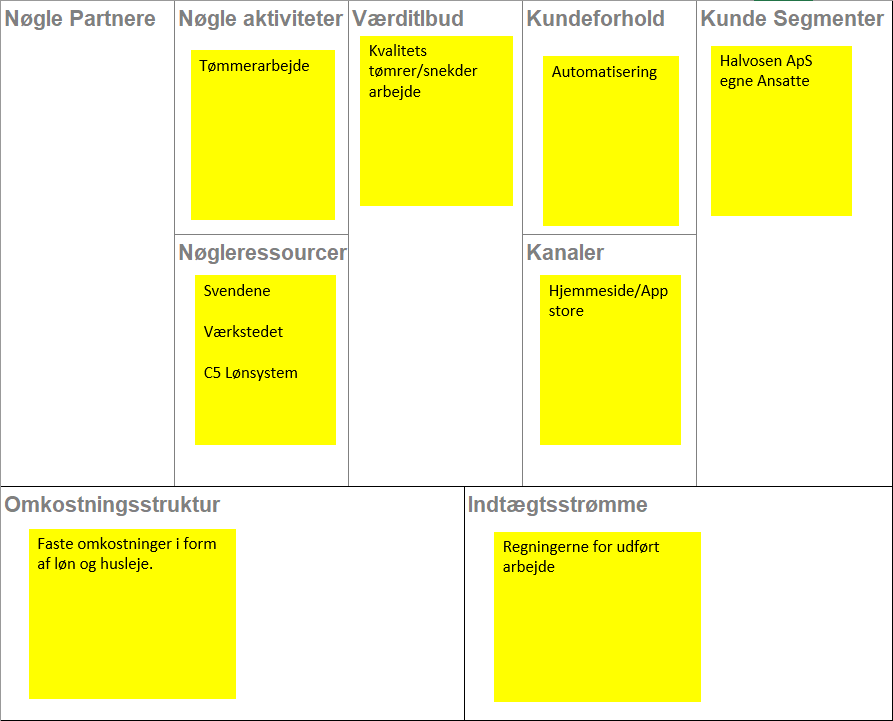
\includegraphics[scale = 0.5]{FML.png}
    \label{forretningsmodelfigur}
\end{figure}
